\section{Features and Functionality}

\subsection{Scene}

\subsubsection{Predefined Scenes/locations}
This feature provides two predefined locations: Ålesund and Uppsala. The Ålesund location covers the Lerstad area in Norway, while the Uppsala location corresponds to Sävja area in Sweden. 

You have the option to create a new location, by inputing the lattitude and longitude of your chosen site, which you can find from Google Maps. Figure \ref{ntnu} provides an example with coordinates corresponding to NTNU in Ålesund. With camera adjustment, you will see the location on the right side of Figure \ref{ntnu}. 

\begin{figure}[H]
    \centering
    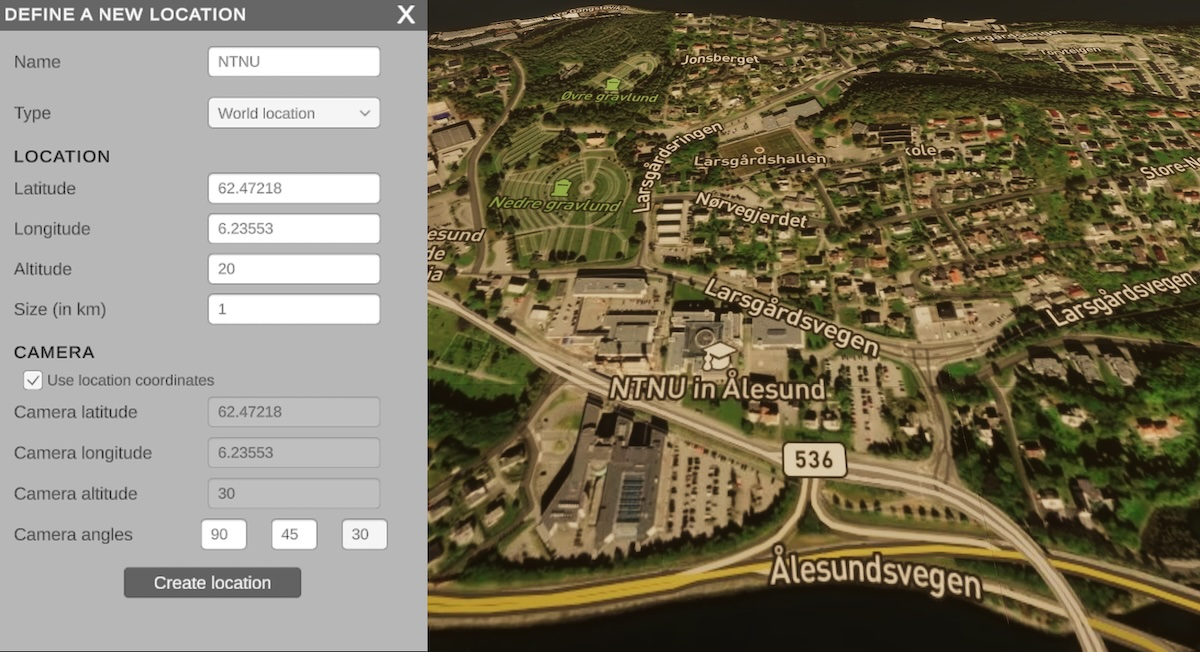
\includegraphics[width=0.98\textwidth]{Images/ntnu.jpg}
    \caption[An example of creating a new location]{An example of creating a new location. Left: the required information to define a new location. Right: the created location with some adjustment on the camera postion}
    \label{ntnu}
\end{figure}

This feature also offers 15 options for customizing the ground appearance, including streets, outdoors, dark, light, satelite, satelite street, commercial, farmland, forest, grass, path, residential, roads, water, and wetland. You can choose to include or exclude the buildings by checking the box of \textit{Display buildings}. All these options are illustrated in Figure \ref{ground}. Note that the ground customization is only applicable to created locations and does not affect the Ålesund and Uppsala locations. Moreover, you have the option to delete the selected location. 

\begin{figure}[H]
    \centering
    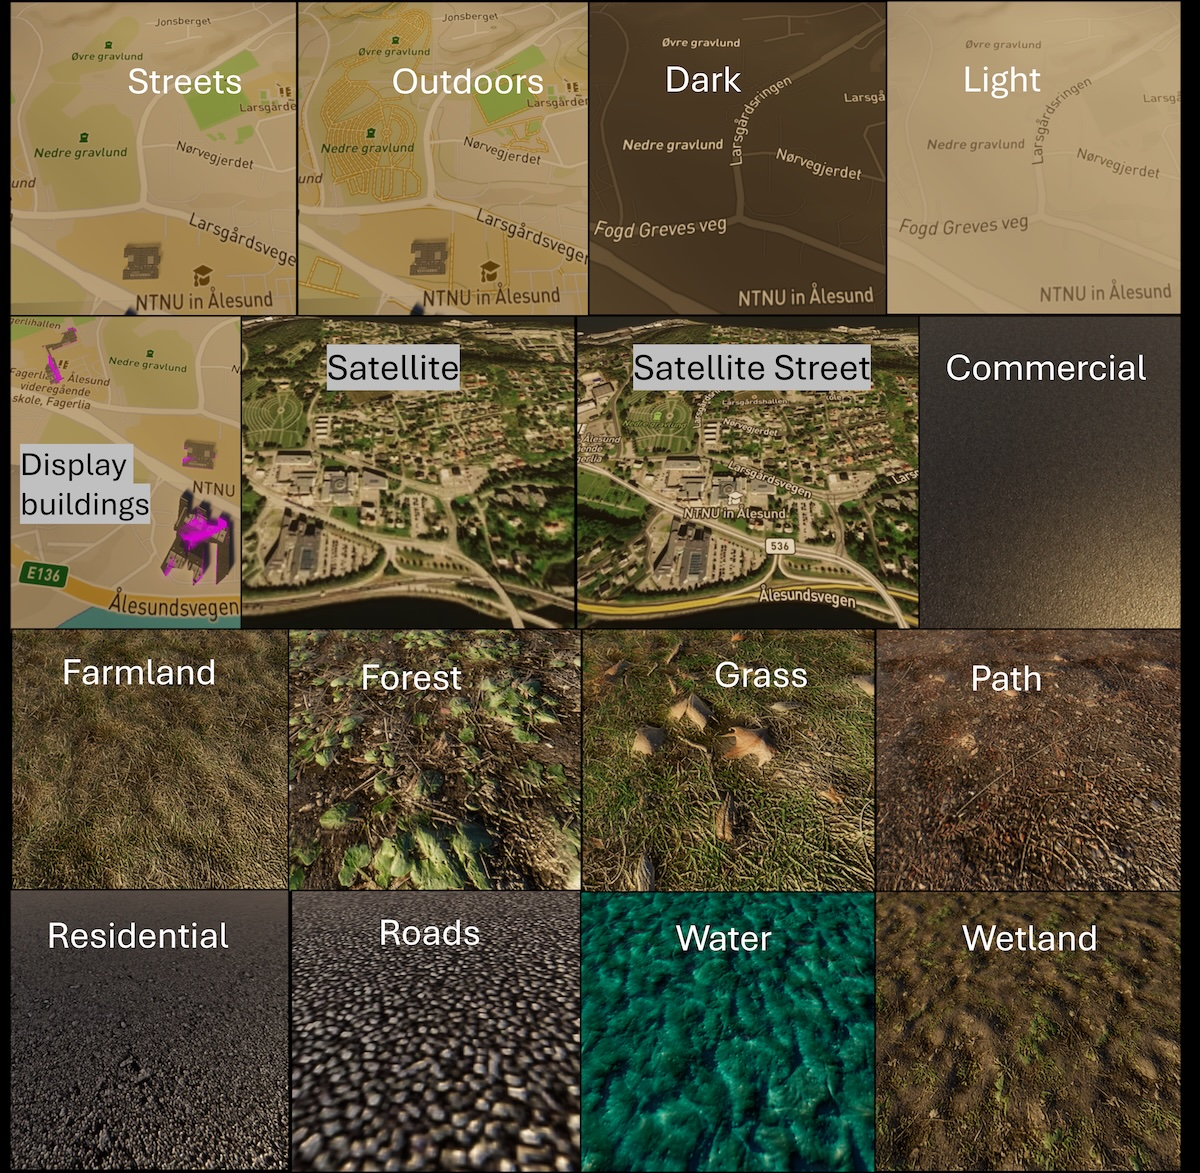
\includegraphics[width=0.98\textwidth]{Images/ground.jpg}
    \caption[Ground option]{Ground option}
    \label{ground}
\end{figure}

Since the sun and moon positions change over time, you can set the desired time by adjusting the hour, date, month, and year. Figure \ref{time} provides an example showing how the sun's position varies depending on the month. In this example, the Ålesund location is shown at the same hour and date for each month.

\begin{figure}[H]
    \centering
    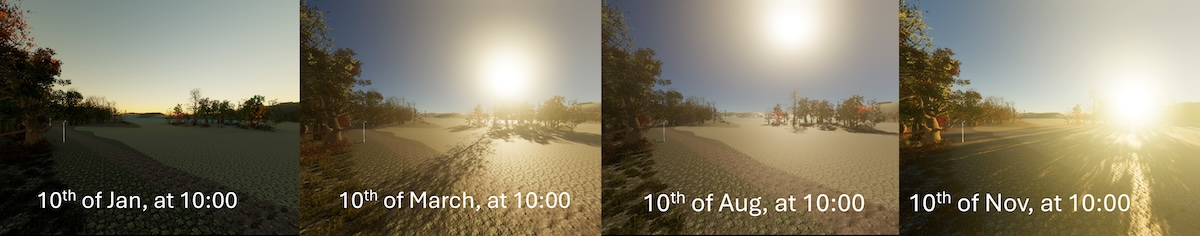
\includegraphics[width=0.99\textwidth]{Images/time.jpg}
    \caption[Sky option]{Sky option}
    \label{time}
\end{figure}

In the \textit{Weather} column, the Scene feature provides five cloud types: clear, sparse, cloudy, overcast, and stormy. You can also customize weather conditions, such as rain, snow, and fog, with intensity level ranging from 0 to 1. 

\subsection{Vegetation} \label{Vegetation_tab}

% Dont understand the biome areas and display nodes 

Vegetation feature covers the vegetation options, such as \textit{Biome areas} and \textit{Vegetation objects}.
The \textit{Display nodes} is to show the ...

You can customize the forest density by adjusting the density bar ranging from 0 to 1. Figure \ref{density} shows the appearance of the forest in Uppsala with different density settings. 
\begin{figure}[H]
    \centering
    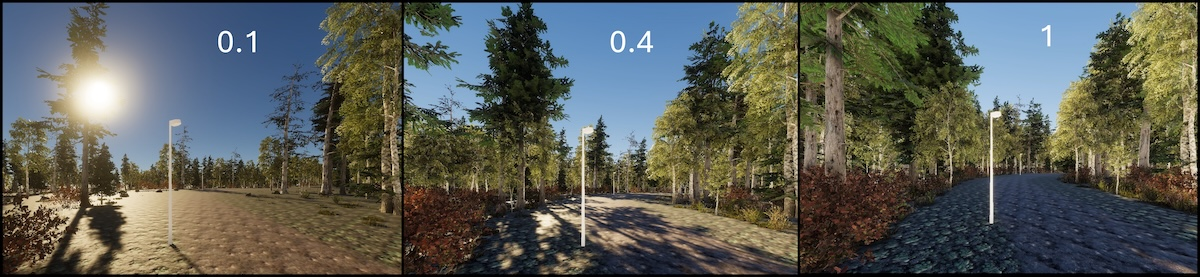
\includegraphics[width=0.99\textwidth]{Images/density.jpg}
    \caption[Density scale in Uppsala]{Density scale in Uppsala}
    \label{density}
\end{figure}

In the \textit{Vegetation objects}, you can create a custom area with six different types of 3D vegetation models. To add a tree, click the \textit{add} button or press the "I" keyboard, then left-click to place the tree. You can adjust the tree's rotation and change its vegetation type. To move a tree, click the \textit{Move} button or press "M". To delete a selected tree, click \textit{Delete} button or press the "Delete" key. Once you have finalized the position, type, and rotation, press "Esc" to deselect the tree. To select a different tree, click on the trunk rather than the leaves. If you want to select multiple trees, hold "Ctrl" while clicking additional ones.

\subsection{Lights} \label{Lights_tab}
Light feature covers illumination from light poles. Several pre-made light poles are available, or you can create your own. To select an existing light pole, you can either (i) click on it directly, or (ii) click the \textit{select} button then double-click the desired pole. The selected pole(s) is marked with a pyramid on the pole, as shown in Figure \ref{selected}.
\begin{figure}[H]
    \centering
    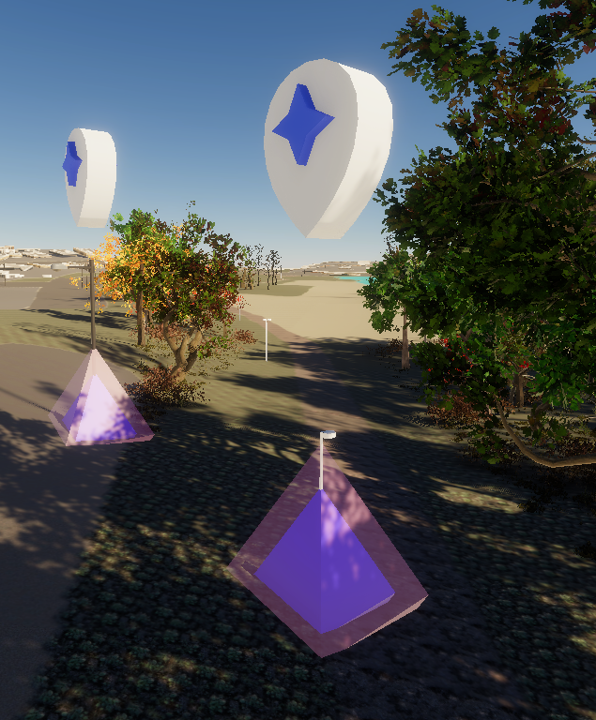
\includegraphics[width=0.75\textwidth]{Images/selected.jpg}
    \caption[Marking the selected poles]{Marking the selected poles}
    \label{selected}
\end{figure}

To add more light poles on the selected scene, use the \textit{add} buttons or press "I" keyboard, then left-click to replace the light pole. You can customize the height and rotation of the selected pole. To move the selected pole, click the \textit{Move} button or press "M". To delete the selected pole, click \textit{Delete} button or press the "Delete" key. Once you have finalized the position, height, rotation, and the model, press "Esc" to deselect the pole. If you want to select multiple poles, hold "Ctrl" while clicking additional ones.

This feature provides 6 different types of 3D-modelled lights, as shown in Figure \ref{light}. The top section shows the light during the day, while the bottom section shows them at night. We provide four types of IES file. IES file defines how light from a lamp is distributed in a space. This data is provided by many manufacturers so that lighting designers can realistically simulate how a project will look when a specific light source is used \cite{IES}. You also have the option to upload your own IES file to customize the lighting.

The \textit{Highlight light poles} checkbox highlights all available light poles. However, to view the result properly, you need to zoom the camera out; otherwise, only a yellow glow will be visible. The \textit{Display light poles} checkbox shows all available light poles, including both default and customized ones. 


\begin{figure}[H]
    \centering
    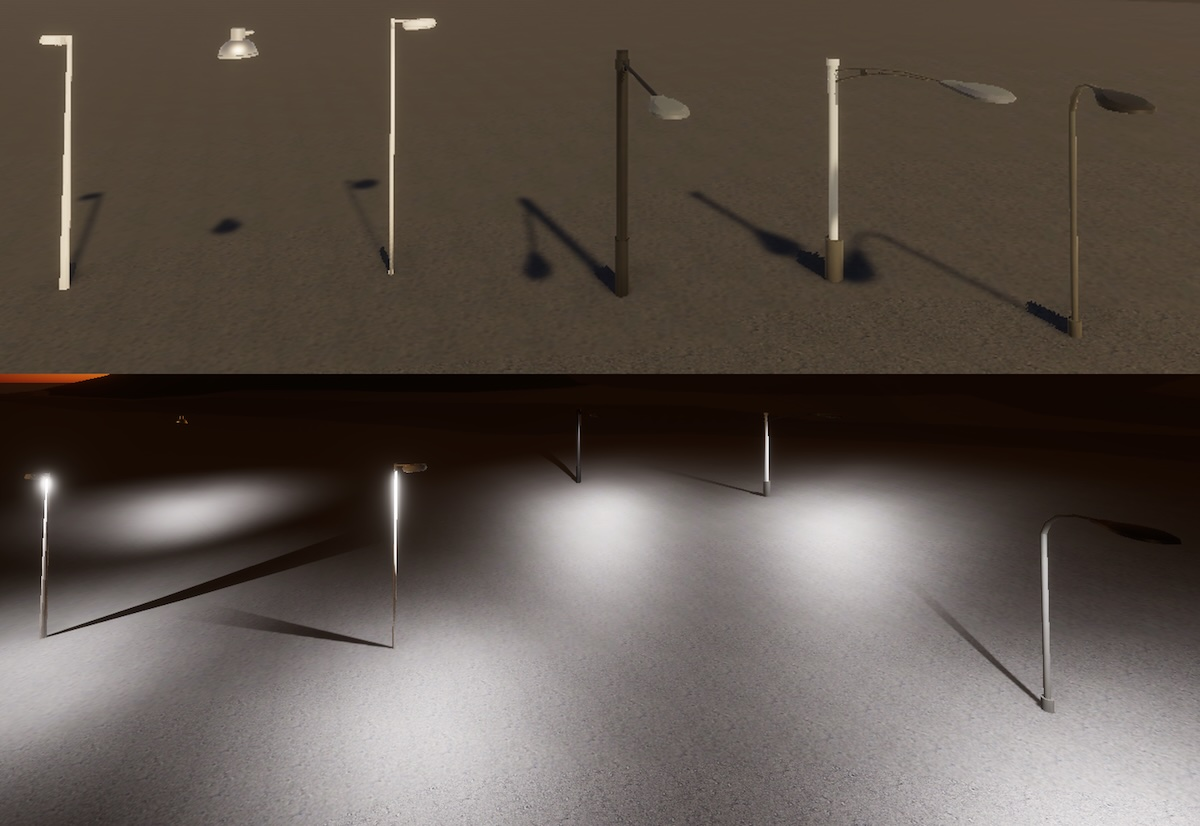
\includegraphics[width=0.99\textwidth]{Images/light.jpg}
    \caption[3D model of light poles]{3D model of light poles. Upper: on the day light. Bottom: on the night}
    \label{light}
\end{figure}

\subsection{Cameras}

Camera feature allows you to manage camera settings, including properties such as sensor size, ISO, shutter speed, lens length, and aperture. You can also add, remove, and modify cameras. To add a camera, click the \textit{Add a new camera} button and specify the camera properties. Note that the most recent settings will be automatically saved to the selected camera. The \textit{Update the current camera position} button adjusts the view in the \textit{Camera preview} to match your screen’s view. On the other hand, the \textit{Move to the current camera position} button changes the view on your screen to match the one in the \textit{Camera preview}. You can also delete the selected camera if needed. 


\subsection{Street View} \label{Street_tab}

The \textit{street view} feature allows users to walk in the scene as if person would do. Follow these steps to use it: (1) adjust the camera to frame the desired scene, (2) press the "Esc" key to release the camera, (3) select a character from the three available options: insect, child, or adult, with heights ranging from 2 cm to 188 cm. %super power???
To readjust the camera, press "Esc" again. Note that in this feature, the "Q" and "E" keys, using to move up and down, do not work. 

\subsection{Light Computation} \label{Computation_tab}

This feature provides the luminance computation. The luminance is a photometric measure of the luminous intensity per unit area of light traveling in a given direction. It is expressed in candela per square meter (cd/m2). In Unity, the luminance is computed from the pixel color and the camera exposure.Three methods are available for visualizing luminance: a luminance map, a luminance graph along a line, and a luminance heatmap in a rectangle. 

To visualize the luminance on the map, explore \textit{luminance map} column and check the \textit{Display luminance map} box. You also have the option to include or exclude the \textit{Log scale}, as shown in Figure \ref{map}. The luminance map will update based on the selected time and season. To check the luminance at a specific point, hover your cursor over the desired location. The luminance value for that point will appear in the \textit{Luminance Map} column under the \textit{Log scale} checkbox. 
\begin{figure}[H]
    \centering
    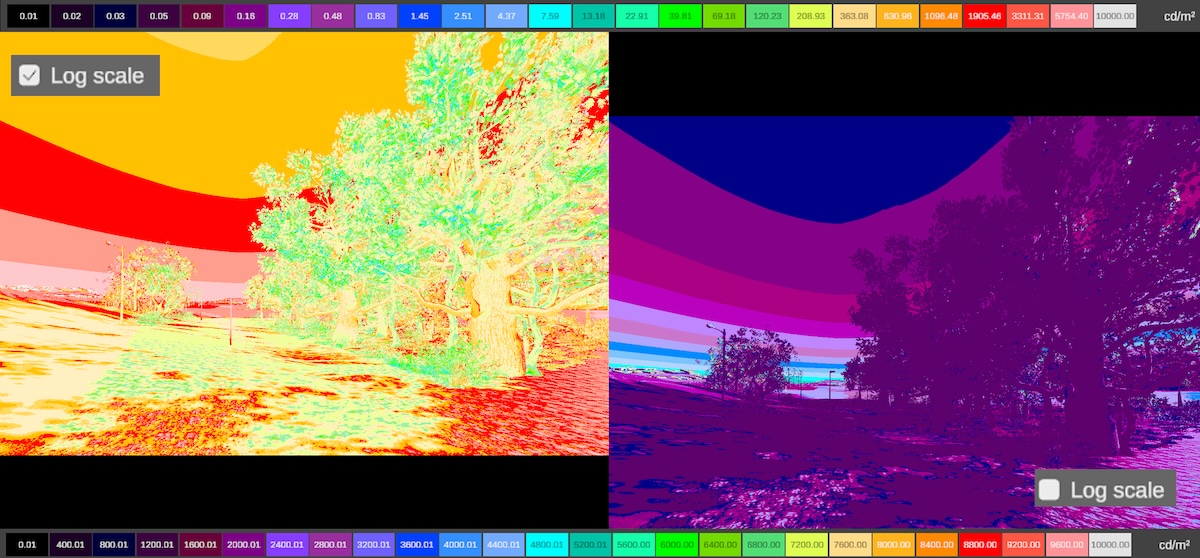
\includegraphics[width=0.99\textwidth]{Images/map.jpg}
    \caption[Luminance map on Ålesund]{Luminance map on Ålesund with log scale (left) and without log scale (right)}
    \label{map}
\end{figure}

To visualize the luminance in a graph, explore the \textit{Line Visualization} column. First, you need to create a line using one of the two methods: 
\begin{itemize}
    \item \textit{Create measure line manually}: click the button to start drawing the line. Place the cursor where you want the line to start, left-click for the starting point, and right-click for the ending point. To create a connected line with multiple segments, continue left-clicking until you're done, then right-click to release the line drawing. 
    \item \textit{Create measure line around light pole}: click the button and select a light pole. You'll need to input three variables for the line: length, angle relative to the light pole, and distance between measurement points. For example, if you want the line to be 10 meters long and take measurements every meter, set the distance to 1 meter. 
\end{itemize}
Next, check the \textit{Display graph} box to show the graph along the drawn line. Figure \ref{graph} provides an example with the blue circle showing two options for visualizing luminance: column graph and line graph.
\begin{figure}[H]
    \centering
    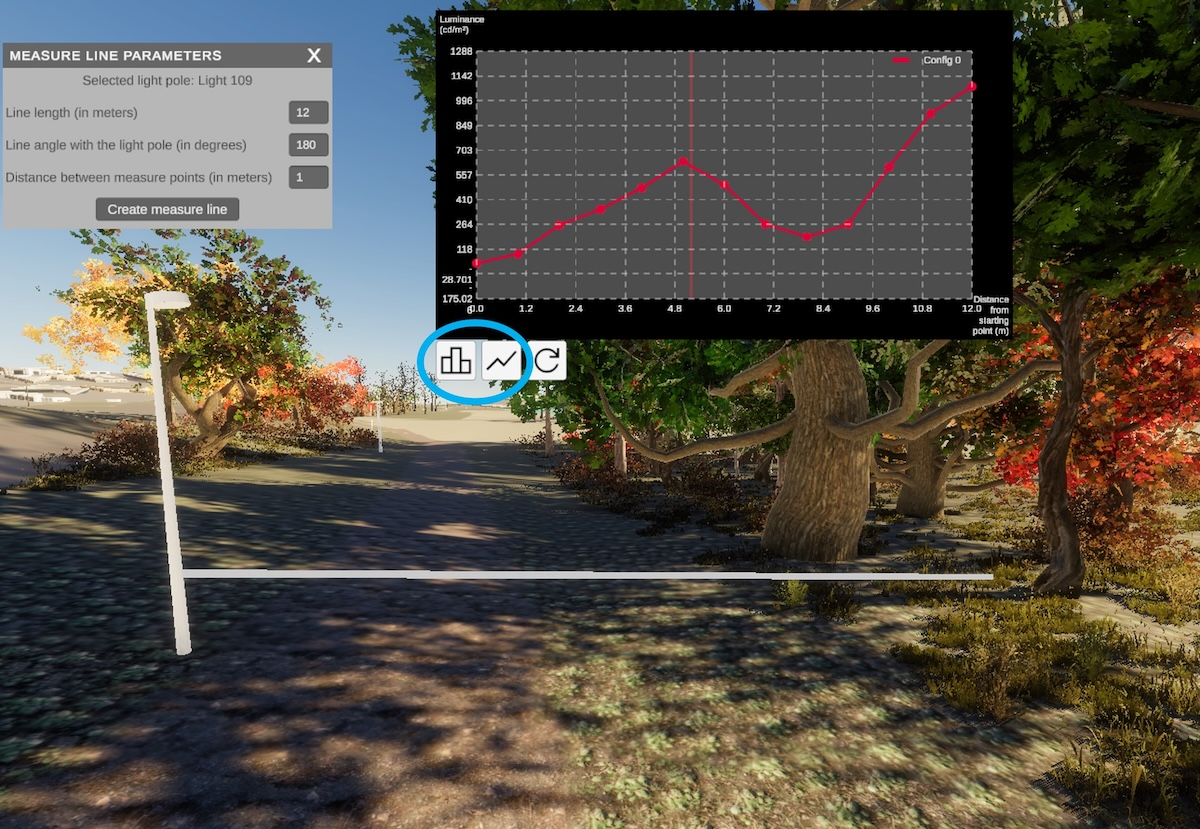
\includegraphics[width=0.99\textwidth]{Images/graph.jpg}
    \caption[One example of visualizing the luminance in line graph]{One example of visualizing the luminance in line graph}
    \label{graph}
\end{figure}
%how to delete the line?

To visualize the luminance as a heatmap, explore the \textit{Grid Visualization} column. First, you create a rectangle by clicking the \textit{Create measure rectangle} button, then position the cursor of where you want the rectangle. Start the drawing by left-clicking, adjust the size as needed, then release the drawing with a right-click. Next, check the \textit{Display heatmap} box. If you want to view the location of a certain heatmap, bring the cursor on the heatmap. A red line will appear within the rectangle, indicating the location. Figure \ref{heatmap} provides an example, showing the cursor on the heatmap and the red line in the rectangle, captured with a phone camera. You can also include or exclude the values on the heatmap using the checkbox \textit{Display values on heatmap}.

\begin{figure}[H]
    \centering
    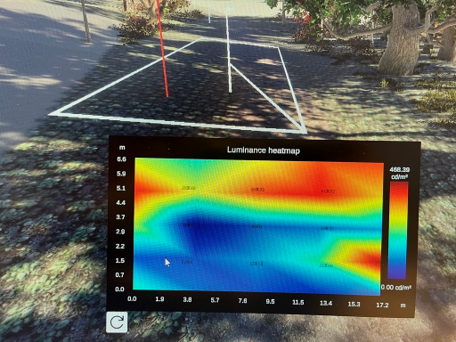
\includegraphics[width=0.99\textwidth]{Images/heatmap.jpg}
    \caption[One example of luminance heatmap]{One example of luminance heatmap, showing the cursor on the heatmap and a red line on the rectangle }
    \label{heatmap}
\end{figure}

You can save the luminance results (graph and heatmap) by exporting them as GeoJSON and CSV files. For graph visualization, you can later import the saved results to compare them with new ones. 

In the \textit{Configurations} column, you can split the screen into up to four sections. This is useful for comparing luminance maps across different settings. An example of this can be seen in Figure \ref{config}, where the reference pole is highlighted with a yellow circle. The top-left section shows the default setup with only two light poles. The top-right section has no light poles in the area. The bottom-left section includes four light poles, three of which are positioned toward the left side. The bottom-right section also shows four light poles, but three are positioned toward the right side. The image was captured during the same setup at midnight.

\begin{figure}[H]
    \centering
    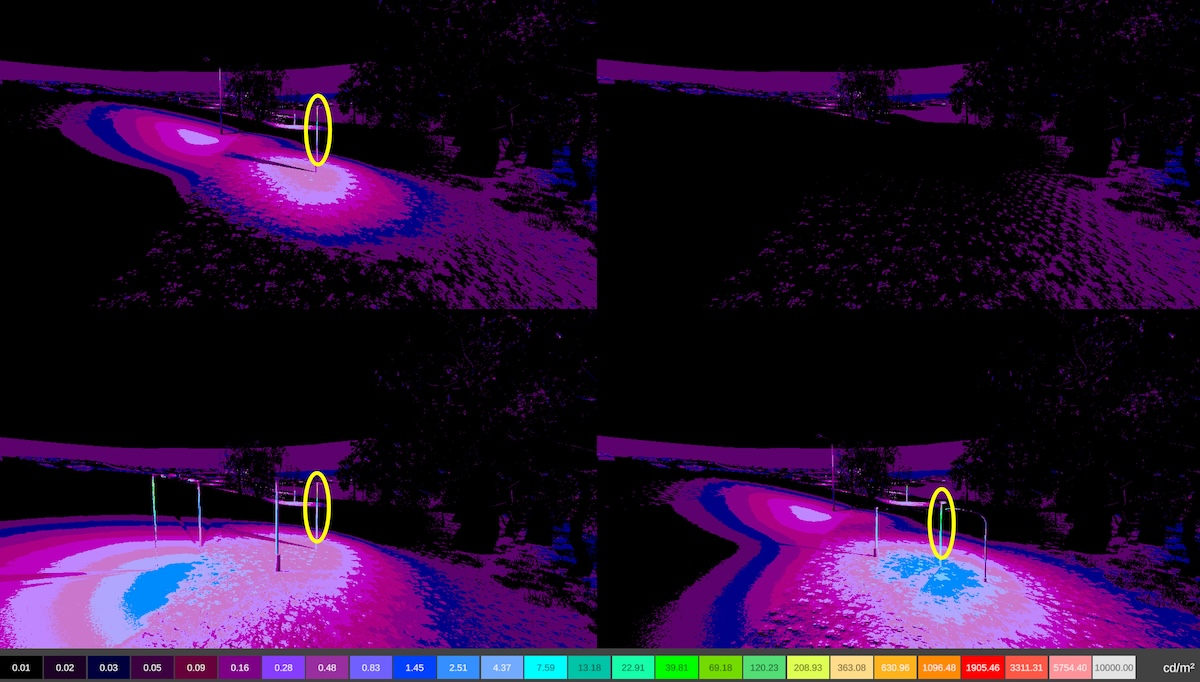
\includegraphics[width=0.99\textwidth]{Images/config.jpg}
    \caption[Luminance map comparison for four configurations]{Luminance map comparison for four configurations}
    \label{config}
\end{figure}

\subsection{Data Visualization} \label{datavis}

This feature supports visualization exclusively for data in the GeoJSON format. This format requires a geometry property that defines the data's location. The geometry can be represented as either a Point or a LineString, both using latitude and longitude coordinates. These coordinates can be obtained via Google Maps or by following the steps outlined in Section \ref{converting}. The feature visualizes data by scaling values between 0 and 1, displayed in a heatmap and a bar chart. In this context, 0 (shown in red) represents the lowest or worst value, while 1 (shown in blue) indicates the highest or best. Therefore, the data you want to visualize must be quantitatively scalable. If your dataset consists of qualitative descriptions that cannot be translated into a numerical value, it cannot be visualized using this feature. An example of compatible data is provided, which is the walkability analysis of different paths in the Ålesund area.

First, you need to download a file named "Path1mDATAStudyCase2WGS84.geojson". Then, on the \textit{Data visualization} feature, click the \textit{Add dataset} button, and select the file. With screen adjustments, the final view appears as shown in Figure \ref{WGS84}. At the bottom, you see a heatmap bar ranged from red (0) to blue (1). This heatmap indicates the walkability in different path based on the selected scenario. The red areas represent the most challenging sections, while orange, yellow, green, and blue indicate progressively easier terrain.
\begin{figure}[H]
    \centering
    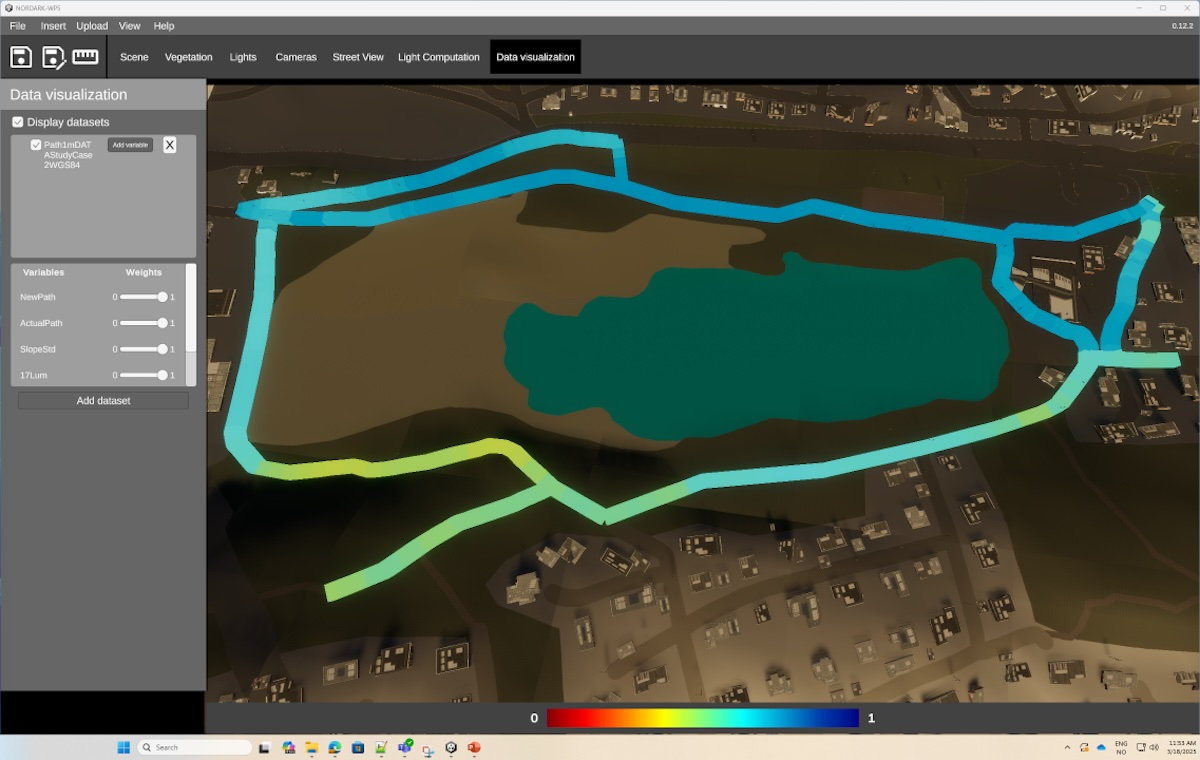
\includegraphics[width=0.99\textwidth]{Images/WGS84.jpg}
    \caption[An example of data visualization]{An example of data visualization}
    \label{WGS84}
\end{figure}

On the left side of Figure \ref{WGS84}, you will find several variables with adjustable weights ranging from 0 to 1, including \textit{NewPath, ActualPath, SlopeStd, 17Lum, 5Lum,} and \textit{ActualLum}. Modifying these variables allows you to customize the desired scenario. To better understand these variables, we provide Figure \ref{abcdef}. 
\begin{itemize}
    \item \textbf{(a)}. The difficulty level is assessed based on the actual path, reflecting real ground conditions.
    \item \textbf{(b)}. The assessment focuses solely on the slope condition.
    \item \textbf{(c)}. The difficulty level is evaluated considering the actual lighting conditions.
    \item \textbf{(d)}. The analysis incorporates three variables simultaneously: actual path, slope condition, and actual lighting.
    \item \textbf{(e)}. While considering the actual path and slope condition, the light condition is adjusted to 17 and 5 luminance
    \item \textbf{(f)}. The difficulty level is assessed using the slope condition in combination with the new path. The new path includes modifications to both ground and lighting conditions, aiming to make the entire area more walkable.
\end{itemize}
\begin{figure}[H]
    \centering
    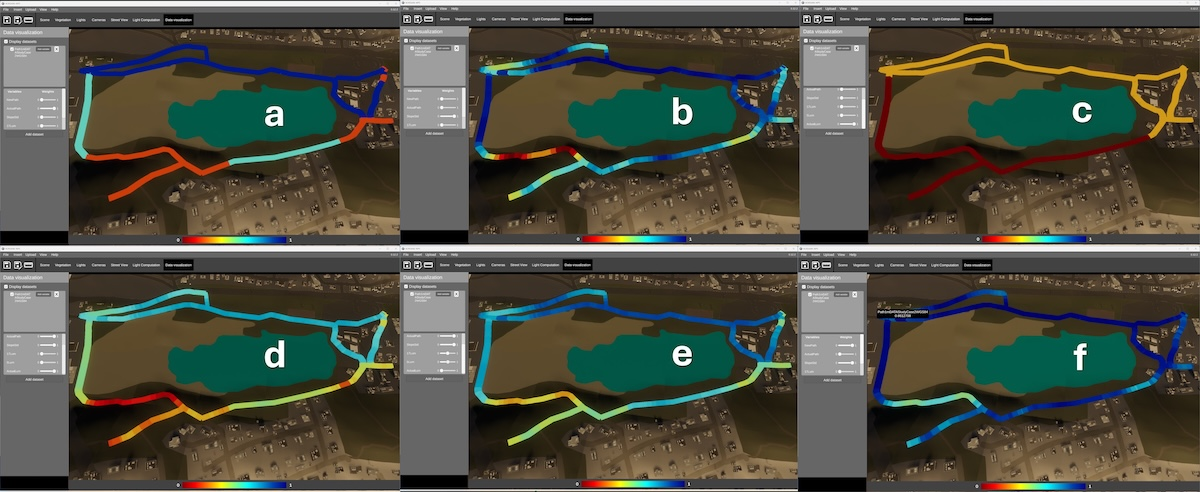
\includegraphics[width=0.99\textwidth]{Images/abcdef.jpg}
    \caption[Data visualization on the walkability based on the considered varibles]{Data visualization on the walkability based on the considered varibles. (a) considering the actual path, (b) considering the slope condition, (c) considering the actual lighting condition, (d) considering the actual path, the slope condition, and the actual lighting, (e) considering the actual path and slope condition, while adjusting the light condition with 17 and 5 luminance, (f) considering the slope condition with the new path.}
    \label{abcdef}
\end{figure}






